%!TEX root = ../template.tex
%%%%%%%%%%%%%%%%%%%%%%%%%%%%%%%%%%%%%%%%%%%%%%%%%%%%%%%%%%%%%%%%%%%%
%% chapter4.tex
%% NOVA thesis document file
%%
%% Chapter with lots of dummy text
%%%%%%%%%%%%%%%%%%%%%%%%%%%%%%%%%%%%%%%%%%%%%%%%%%%%%%%%%%%%%%%%%%%%
\chapter{Casos de Estudo}
Neste capítulo iremos analisar possibilidades de uso da linguagem. Alguns desses exemplos são até já parcialmente ou totalmente funcionais quando executados pelo interpretador de referência desenvolvido nesta dissertação. Outros exemplos fazem uso de funcionalidades planeadas mas ainda não implementadas, e que serão devidamente identificados quando necessário.
Nestes exemplos podem também ser usados pequenos excertos de músicas para demonstrar a utilização da linguagem, e a forma como esses excertos podiam ser representados com a nossa sintaxe. Estes casos de estudo não são apenas uma forma de mostrar como os vários componentes da aplicação funcionam em conjunto, mas são também uma forma de ilustração da linguagem. É muitas vezes mais fácil decidir qual a melhor forma de implementar uma funcionalidade quando temos vários casos de estudo de qual é a forma que podemos tirar melhor proveito da mesma.

\section{Tocar Música}
\label{casestudies:westworld}
\begin{lstlisting}[caption=Exemplo da sintaxe para criação de música,language=PHP]
# Title: Westworld Main Theme

:piano = I1 S6/8 T70 L/8 V120;
:violin = :piano(I41);

$chorus = :piano (A*11 G F*12 | A,6 A,5 G, F,6*2)*3;

$melody = :piano (r24   (:violin a3 c'3 d'3 e'9) r9 e'3 d'3 c'3 a9);

play( $chorus | $melody );
\end{lstlisting}

% TODO Add back
%\includemovie[text=\underline{Clicar para Reproduzir Aúdio}, attach=false]{}{}{../../code/SoundPlaygroundPy/examples/westworld.wav}

Nas duas primeiras linhas deste exemplo podemos verifica a utilização de duas vozes (\texttt{:piano} e \texttt{:violin}). O piano ocupa a posição 1 da \textit{soundfont} utilizada, enquanto que o violino utiliza a posição 41. Ao declarar o piano, podemos também definir um conjunto de configurações adicionais (como o compasso, a duração base das notas, e o volume com que são tocadas). Ao declarar o violino, podemos herdar as configurações de outro instrumento (neste caso o piano) e mudar apenas o necessário (a posição do instrumento).

Depois podemos ver a utilização de variáveis (\texttt{\$chorus} e \texttt{melody}) para estruturar e guardar conjuntos de notas, neste caso.
É possível ver também o quão conciso fica descrever padrões ou conjuntos de notas repetidas através do operador de repetição (\texttt{*}). O operador de paralelo (\texttt{|}) permite depois tocar notas em paralelo ao mesmo tempo.

\section{Fuga de Duas Vozes}
\label{casestudies:fugue}
O caso de estudo anterior mostra como é possível declarar algumas notas, e aproveitar operadores simples como a repetição para reduzir a redundância no código. Neste caso de estudo usamos conceitos mais avançados e vemos como podemos declarar uma função, que usa as suas variáveis em mais do que um sítio e de diferentes formas para produzir o resultado final.
\begin{lstlisting}[caption=Exemplo da declaração da estrutura e conteúdo de uma simples fuga de duas vozes,language=PHP]
# Fugue 2 in C minor in Book I of the J.S. Bach’s Well-Tempered Clavier
fun fugue ( $subj, $resp ) => 
    ( $subj $resp | r ** $subj ( $subj + 7 ) );

S8/4 T140 L/4 V120;

$subj = r c/2 B/2 c G _A c/2 B/2 c d
        G c/2 B/2 c d F/2 G/2 _A2 G/2 F/2;

$resp = _E/2 c/2 B/2 A/2   G/2 F/2 _E/2 D/2   C _e d c
        _B A _B c   ^F G A ^F;

play( fugue( $subj, $resp ) );
\end{lstlisting}

Também nos permite analisar que as músicas podem conter estruturas não imediatamente óbvias à primeira vista. A função recebe dois excertos musicais \texttt{\$subj} e \texttt{\$resp}, e toca-os em sequência. Além disso, durante o terceiro e quarto compassos, também toca em paralelo uma versão do \texttt{\$subj} transposta 7 semitons. 

Este é apenas um pequeno exemplo do tipo de transformações e operações que podem ser efetuadas de modo não destrutivo sobre os acompanhamentos musicais. Se quisermos mudar alguma nota em \texttt{\$subj}, quando reproduzirmos o ficheiro novamente, essa alteração irá refletir-se automaticamente na versão transposta também.

\begin{figure}[ht]
  \centering
  {%
  \setlength{\fboxsep}{0pt}%
  \setlength{\fboxrule}{0pt}%
  \fbox{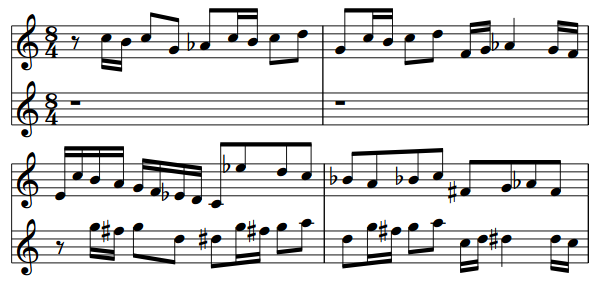
\includegraphics[width=.85\linewidth]{../../code/musikla/musikla/examples/paper/fugue.png}}%
  }%
  \caption{Pauta musical gerada pela linguagem, versão áudio disponível \href{https://drive.google.com/file/d/1dIfvnhhKn73Vpp0W6ss6RLsv6PQ_HFTF/view}{\underline{aqui}}\protect\footnotemark.}
  \label{fig:fugue}
\end{figure}

\footnotetext{Fuga \url{https://drive.google.com/file/d/1dIfvnhhKn73Vpp0W6ss6RLsv6PQ_HFTF/view}}


\section{Definir um teclado}
No início do capítulo \ref{casestudies:westworld} e \ref{casestudies:fugue} podemos ver um pequeno excerto de música que é tocada autonomamente pela linguagem. Aqui poderemos ver como construir um teclado virtual personalizado para tocar essa música, bem como a sequência de teclas a premir para a reproduzir.
    
\begin{lstlisting}[caption=Exemplo da sintaxe para criação de teclados,language=PHP]
# Title: Soft to Be Strong
# Artist: Marina
V70 L1 T120;

fun toggle_sustain ( ref $enabled ) {
    if $enabled then cc( 64, 0 ) else cc( 64, 127 );

    $enabled = not $enabled;
};

$sustained = true;

@keyboard hold extend {
    a: [^Cm];   s: [BM];    d: [AM];    f: [EM];   g: [^Fm];
};

@keyboard hold extend (V120) {
    1: ^c;    2: ^d;    3: e;     4: ^f;   5: ^g;
    6: b;     7: ^c';   8: ^d';   9: e';

    c: toggle_sustain( $sustained );
};
\end{lstlisting}
% TODO Add back
% \includemovie[text=\underline{Clicar para Reproduzir Aúdio}, attach=false]{}{}{../../code/SoundPlaygroundPy/examples/marina.wav}

A sequência de teclas a ser premida neste exemplo é: \textbf{\texttt{A 5 5 5 4 S 3 2 1 D S A 5 6 7 D 7 7 6 S 6 9 8 9 6 7}}. Os tempos de cada tecla são relativamente uniformes e podem ser facilmente deduzidos ouvindo a versão sonora deste extrato musical, disponível \href{https://drive.google.com/file/d/1ncy4vlCbbiGQ14lurfsU4LCCUBK0ve13/view?usp=sharing}{aqui}\footnote{Soft to Be Strong \url{https://drive.google.com/file/d/1ncy4vlCbbiGQ14lurfsU4LCCUBK0ve13/view?usp=sharing}}.

No início deste exemplo podemos ver a declaração de uma função \textbf{toggle\_sustain}, que recebe como parâmetro uma variável por referência. O que isto significa é que qualquer alteração ao valor da variável dentro desta função, reflete-se também na variável que for passada à função quando esta é chamada. 

Na definição da função fazemos uso da função \texttt{cc} que permite controlar diversos controlos \acrshort{midi}. Neste caso, o controlo \textit{64} refere-se ao pedal de \textit{sustain} de um piano (que deixa as notas a tocar durante mais algum tempo mesmo depois da sua tecla ser levantada). O valor 0 (\textit{zero}) que lhe é passado significa desligar esse pedal, e o valor \textit{127} significa ligar esse pedal. Apesar de ser sempre possível recorrer a este tipo de funções de baixo nível, são também disponibilizadas na biblioteca \textit{standard} as funções mais comuns (como por exemplo, \texttt{sustainoff()} e \texttt{sustainon()}).

Depois podemos ver a declaração de dois teclados virtuais (a linguagem permite mais do que um teclado ativo ao mesmo tempo). O primeiro mapeia a algumas teclas (\texttt{a, s, d, f e g}) o conjunto de acordes usados nesta música. Para além disso também define alguns modificadores a serem usados por este teclado (cujo significado é discutido na sub-secção \ref{modifiers}).

O segundo teclado funciona de forma similar, atribuindo às teclas de 1 a 9 notas individuais a serem tocadas. Neste teclado podemos também ver que notas musicais não são os únicos elementos que podem ser associados a teclas. Também é possível descrever expressões arbitrárias (como neste caso, a chamada da função \texttt{toggle\_sustain( \$sustained )} associada à tecla \textbf{c}).

Outro ponto a notar sobre o segundo teclado é a declaração entre parênteses \texttt{(V120)} que permite modificar o volume das notas tocadas por este teclado (que se sobrepõe ao volume global \texttt{V70} indicado no início do código). Isto é uma forma simples de prefixar configurações a todas as notas do teclado, evitando ter de copiar essas configurações para todas as notas.

\section{Teclado de \textit{Arpeggios}}
Neste exemplo vamos construir um teclado mais dinâmico. Vamos associar a algumas teclas diferentes acordes. Mas em vez de tocar simplesmente esses acordes, vamos tocá-los como arpeggios aplicados a um padrão.

É importante notar que o padrão não está escrito estaticamente, mas sim guardado na variável \texttt{\$pat}. Isto significa que podemos depois usar um segundo \textit{keyboard} para controlar qual o padrão ativo. E para tornar o exemplo ainda mais divertido, usamos as setas \textit{up} e \textit{down} para aumentar ou diminuir a transposição das notas resultantes, dando assim mais variedade aos quatro acordes definidos.

É fácil de ver também como este teclado é extremamente versátil, e pode ser facilmente adaptado para um qualquer número de acordes e \textit{arpeggios} que se queira utilizar.

\begin{lstlisting}[caption=Definição de um teclado de acordes,language=PHP]
S4/4 L/4 T132 V120;

$patterns = @[
    C D E D2 E C2;
    C r d' e2 r c2;
];

$t = 0; $pat = $patterns::[ 0 ];

@keyboard {
    a: [CM];
    s: [Am];
    d: [FM];
    f: [Dm];
}::map(fun($k, $m) => $m * $pat + $t);

@keyboard {
    1: { $pat = $patterns::[ 0 ] };
    2: { $pat = $patterns::[ 1 ] };

    up: { $t += 1 };
    down: { $t -= 1 };
};
\end{lstlisting}

\section{Teclado Geral com MIDI}
Os dois teclados vistos até agora são interessantes quando temos um sub-conjunto específico de notas e acordes com os quais queremos tocar. Mas às vezes é interessante ter uma ferramenta mais genérica para experimentar.

Este exemplo faz uso de funções disponibilizadas na biblioteca \textit{standard} da linguagem para fazer isso mesmo. 

\begin{itemize}
 \item \texttt{keyboard\textbackslash{}piano()} Cria um teclado a simular um piano com as teclas do computador. A primeira linha de teclas corresponde às teclas brancas, a segunda às teclas pretas e a terceira novamente às brancas mas uma oitava acima.
 \item \texttt{keyboard\textbackslash{}midi()} Cria um teclado que está à escuta dos eventos MIDI (possivelmente de um piano externo ligado ao computador).
 \end{itemize}
 
 De seguida também vemos que é possível fazermos \textit{override} a algumas teclas se quisermos algo mais específico. Isto é opcional e pode ser ignorado se quisermos.
 
 \begin{itemize}
  \item \texttt{keyboard\textbackslash{}bufpad()} Aqui criamos um teclado que está à escuta das teclas numéricas (de 1 até 9) e cria um \textit{buffer} em cada uma delas. Podemos usar esses \textit{buffers} para guardar em memória melodias que toquemos com os teclados, para depois as reproduzir quando quisermos.
 \item \texttt{keyboard\textbackslash{}repl()} Finalmente criamos um último teclado que faz a tecla "\textbackslash{}" ativar o editor embutido. Assim conseguimos alterar o nosso programa enquanto ele está a correr, alterar teclas, mexer nos \textit{buffers}, declarar variáveis ou gravar os resultados das nossas experiências para disco.
\end{itemize}


\begin{lstlisting}[caption=Junção de vários teclados criados usando funções da biblioteca standard,language=PHP]
# Use a "standard" keyboard piano
$piano = keyboard\piano();
# Maybe even add a MIDI piano?
$piano += keyboard\midi();
# Or declare a custom piano
$piano += @keyboard hold extend {
    a: [^Cm];       s: [BM];        d: [AM];
    f: [EM];        g: [^Fm];       
};

# Creates a keyboard that declares a set of buffers. By default, 
# the numpad keys are used (creating 10 available buffer slots)
# Save key is F8, Load key is F7
$piano += keyboard\bufpad();
# Creates a keyboard that associates the interpreter accessible by the "\" key
$piano += keyboard\repl();
\end{lstlisting}

\section{QWERTY Keyboard}
% A função \texttt{qwertyboard} é uma função planeada a ser incluída na biblioteca \textit{standard} da linguagem. Aqui temos um exemplo simplificado do que essa função irá ser.
% Neste exemplo podemos observar funcionalidades mais genéricas da linguagem. Muitas dessas funcionalidades (arrays, métodos de objetos, funções anónimas) ainda não se encontram implementadas na versão atual do protótipo, mas servem como exemplo para o que a linguagem irá no fim permitir.
No exemplo anterior utilizamos as funções fornecidas pela biblioteca \textit{standard}. Aqui vamos ver um exemplo de como poderíamos programar as nossas próprias funções, utilizando funcionalidades mais dinâmicas (como ciclos \texttt{for}) do que simplesmente declarar cada tecla manualmente.

Neste caso estamos a criar um teclado em que cada linha de teclas começa uma oitava acima de onde a linha de baixo começou, e as teclas na mesma linha sobem um semitom cada uma.
\begin{lstlisting}[caption=Exemplo de criação de um teclado de forma dinâmica,language=PHP]
fun qwertyboard () {
    # Small shortcut function
    fun ivl ($o, $s) => interval( octaves = $o, semitones = $i );

    # Maps the lines on a keyboard to semitone offsets to List[ List[ str ] ]
    $lines = @[
        "qwertyuiop"::split(),
        "asdfghjkl"::split(),
        "zxcvbnm,."::split()
    ];
    
    $octave = 0;
    $semitone = 0;
    
    $keyboard = @keyboard hold extend {
        for ( $oct, $chars in enumerate( $lines ) ) {
            for ( $sem, $c in enumerate( $chars ) ) {
                [ $c ]: c + ivl( -$oct, $sem );
            };
        };
    }::map( fun( $k, $events ) => $events + ivl( $octave, $semitone ) );
    
    $keyboard += @keyboard {
        up: { $octave += 1 };
        down: { $octave -= 1 };
        right: { $semitone += 1 };
        left: { $semitone -= 1 };
    };
    
    return $keyboard;
}
\end{lstlisting}
A primeira parte da função declara um \textit{array} com as três linhas de caracteres presentes num teclado \textit{QUERTY}. Isto permite-nos ao declarar as teclas no \textit{keyboard}, e fazê-lo de forma dinâmica (ao invés de associar a cada tecla uma nota manualmente).

Essa declaração, inspirada nas listas por compreensão do \textit{Python}, funciona através de uma construção similar a um ciclo \textit{for}. A variável \texttt{\$c} corresponde a cada item da \textit{linha} (neste caso, casa tecla), a variável \texttt{\$sem} permite-nos obter o índice da letra atual na \textit{linha}. A cada letra é associada a nota \texttt{c} transposta pelo índice da tecla e da linha a que pertence.

Para além disso também podemos ver a declaração de mais quatro teclas (correspondentes às quatro setas do teclado) que permitem deslocar as notas tocadas por oitavas completas ou por semitons. Para isso, estas teclas têm associadas uma expressão de bloco (identificada pelas chavetas \texttt{\{} e \texttt{\}}), que é avaliadano mesmo âmbito lexical da função que as criou sempre que a tecla é premida. Lá dentro é possível meter uma instrução (ou opcionalmente várias, separadas por pontos e vírgulas \textbf{;}). O valor da última expressão é o valor de retorno da expressão de bloco toda, pelo que seria possível que uma tecla fizesse mais que uma coisa (mudar o estado e retornar ainda notas para serem tocadas, por exemplo).

Finalmente vemos também um exemplo do método \texttt{map}, um dos vários métodos que o objeto \texttt{Keyboard} disponibiliza e que permitem modificar ainda mais o comportamento dos teclados, alterando o valor emitido por cada tecla de acordo com a função passada.

\needspace{.2\textheight}

\section{Conclusão}
Com estes exemplos pudemos ver como ter uma sintaxe musical declarativa torna bastante compacta a descrição de acompanhamentos musicais. Mas mais do que poder descrevê-los estaticamente, o facto de podermos repetir e transformar sequências musicais aumenta ainda mais a produtividade do utilizador.

Para além disso também conseguimos observar que a integração dos teclados abre portas para situações bastante interessantes, principalmente quando usados em conjunto com as ferramentas de programação dinâmica disponíveis. Um exemplo disso é o caso do nosso teclado de \textit{arpeggios}, onde podemos definir apenas um conjunto de acordes, e depois aplicar uma transformação comum a todos eles para produzirem expressões mais complexas (que podem ser depender de variáveis que vão mudando ao longo da execução).

Para além disso, também concluímos que é importante que a biblioteca \textit{standard} inclua ferramentas genéricas e prontas a utilizar, tais como teclados com as teclas já preenchidas para os casos de uso mais comuns. Isto é útil para facilitar a utilização da linguagem por pessoas que possam sentir-se à vontade com pequenos \textit{scripts} que mudem algumas variáveis e chamem algumas funções, mas não tenham experiência suficiente para criar tudo de raiz.

Por fim, é também algo importante permitir a execução de código (nem que seja apenas de expressões ou instruções singulares, possivelmente através de um simples \texttt{REPL} (read-eval-print loop) em \textit{runtime}. Isto permite ir refinando o programa, principalmente os teclados que possam estar ativos, sem ser necessário terminar a execução do programa. Obrigar o utilizador a reiniciar a aplicação sempre que quiser efetuar modificações ao código da aplicação, para além de ser uma ação mais demorada, apresenta também a desvantagem de fazer a aplicação perder os dados guardados memória, e como tal perder o estado das variáveis e dos \textit{buffers} que pudessem estar a ser usados.
